\documentclass[11pt,a4paper]{article}

\usepackage[margin=2.5cm]{geometry}
\usepackage{amsmath,amssymb,mathtools}
\usepackage{amsthm}
\usepackage{booktabs,tabularx,array}
\usepackage{enumitem}
\usepackage{microtype}
\usepackage{xcolor}
\usepackage{pgfplots}
\pgfplotsset{compat=1.18}
\usepackage[colorlinks=true,linkcolor=blue!50!black,citecolor=blue!50!black,urlcolor=blue!50!black]{hyperref}

\newcommand{\E}{\mathbb{E}}
\newcommand{\Var}{\mathrm{Var}}
\newcommand{\Cov}{\mathrm{Cov}}
\newcommand{\Wt}{\tilde W}
\newcommand{\xb}{\bar x}
\newcommand{\xtil}{\tilde x}
\newcommand{\upast}{U_{\mathrm{past}}}

\newtheorem{lemma}{Lemma}

\setlist{itemsep=2pt,topsep=4pt}

\title{Neuron-Dropout Faults in Fractional-Order Reservoirs:\\ A Theoretical Analysis}
\author{Navid Shamszadeh}
\date{4 October 2026}

\begin{document}
\maketitle

\begin{abstract}
\noindent
Clamping a neuron's weights to zero acts on a fractional-order reservoir (FOR) as an injected ``anti-signal'': the exact negative of what that neuron used to send. The reservoir's response is that forcing passed through the fractional dynamics. In a linearized model this yields closed-form results with five consequences.
\begin{itemize}
  \item \textbf{The path depends on $\alpha$.} After a permanent fault the reservoir relaxes to its new state as a power law, $t^{-\alpha}$, not exponentially. With an untruncated Gr\"unwald--Letnikov (GL) history there is no characteristic recovery time.
  \item \textbf{The endpoint does not, at a fixed operating point.} Given the neurons' mean rates and gains, the fault's shift of the mean operating point is independent of $\alpha$. With a truncated GL buffer, $\alpha$ and $L$ enter through an effective leak. In a spiking reservoir the rates and gains themselves depend on $\alpha$, so the endpoint does too, but only through them.
  \item \textbf{In hardware, the buffer length matters as much as $\alpha$.} Truncation at $L$ steps caps recovery: for $\tau_m = 10$ steps at about $1.5L$ to $2.5L$ steps, and longer for slower membranes. For short buffers, recovery time peaks at intermediate $\alpha$.
  \item \textbf{Lost memory capacity with a retrained readout is exactly 1 per neuron in the linear, noise-free limit.} That holds for every $\alpha$. Any $\alpha$-dependence of fault tolerance measured with retraining therefore comes from noise, spiking nonlinearity or quantization, which tells you where to look.
  \item \textbf{Random dropout moves the reservoir toward the ordered regime.} The effective coupling gain shrinks by a factor of $\sqrt{1-p}$ when a fraction $p$ of neurons is removed.
\end{itemize}
The derivations use the GL-FLIF model and the information measures of Mastin et al.~\cite{mastin2026}. A numerical check of the main scaling laws is included.
\end{abstract}

%=====================================================================
\section{Model and fault definitions}

The analysis linearizes the spiking GL-FLIF reservoir of Mastin et al.~\cite{mastin2026} into a linear fractional-order network. That model is exactly solvable, and its predictions are then checked against the spiking model.

\subsection{The GL-FLIF reservoir}

Each neuron $i$ follows Algorithm~1 of~\cite{mastin2026}, with Gr\"unwald--Letnikov coefficients $c_k = (-1)^k\binom{\alpha}{k}$ and a history buffer of length $L$:
\begin{equation}
V_{i,n} = \Delta t^{\alpha}\left( -\frac{V_{i,n-1} - V_{\mathrm{rest}}}{\tau_m} + I_{i,n} + b \right) - \sum_{k=1}^{L} c_k \, V_{i,n-k},
\qquad
I_{i,n} = \sum_j W_{ij}\, s_{j,n-1} + \sum_m W^{\mathrm{in}}_{im}\, u_{m,n},
\label{eq:glflif}
\end{equation}
with threshold $V_{\mathrm{th}}$, reset to $V_{\mathrm{reset}}$, spikes $s_j$ and a linear readout $y_n = W_{\mathrm{out}} x_n$. For $0<\alpha<1$, every $c_k$ with $k\ge 1$ is negative and $\sum_{k\ge 0} c_k = 0$. So $-\sum_k c_k V_{n-k}$ is a weighted average of past potentials whose weights $|c_k|$ decay as $k^{-1-\alpha}$. For $\alpha=1$ only $c_1=-1$ survives and the update reduces to the forward-Euler LIF neuron.

\begin{lemma}
  For $0<\alpha < 1$ and $k\geq 1$ every $c_k(\alpha)$ is negative and
  \begin{equation}
    \label{eqn:sum_ck}
  \sum_{k=0}^{\infty} c_k(\alpha) = 0
  \end{equation}
\end{lemma}
\begin{proof}
  We first show the ratio 
  \[
  \frac{c_k}{c_{k-1}} = \frac{k-1-\alpha}{k}
  \]
  To see this we expand $c_k$ and $c_{k-1}$:
  \[
  \frac{c_k}{c_{k-1}} = \frac{(-1)^k{\alpha\choose k}}{(-1)^{k-1}{\alpha\choose k-1}} = -\frac{{\alpha\choose k}}{{\alpha\choose k-1}}
  \]
  Note that for positive non-integer $\alpha$ we use the Gamma function $\Gamma(\cdot)$ for binomial coefficients:
  \[
  {\alpha\choose k} = \frac{\Gamma(\alpha+1)}{\Gamma(k+1)\Gamma(\alpha - k + 1)} \implies -\frac{{\alpha\choose k}}{{\alpha\choose k-1}} = 
  -\frac{\frac{\Gamma(\alpha+1)}{\Gamma(k+1)\Gamma(\alpha - k + 1)}  }{\frac{\Gamma(\alpha+1)}{\Gamma(k)\Gamma(\alpha - k + 2)}}
  \]
  \[
  = -\frac{\Gamma(k)\Gamma(\alpha-k+2)}{\Gamma(k+1)\Gamma(\alpha-k+1)}
  \]
  Note that $\Gamma(z+1) = z\Gamma(z)$ for any complex number with positive real part. Therefore we can simplify in the following manner:
  \[
  -\frac{\Gamma(k)\Gamma(\alpha-k+2)}{\Gamma(k+1)\Gamma(\alpha-k+1)} = -\frac{(\alpha-k+1)\Gamma(k)\Gamma(\alpha-k+1)}{k\Gamma(k)\Gamma(\alpha-k+1)}
  = -\frac{\alpha - k + 1}{k}
  \]
  \[
  = \frac{k-1-\alpha}{k}
  \]
  Let $\rho_k = \frac{k-1-\alpha}{k}$. Then we can write $c_k = \rho_k c_{k-1}$. Applying this recursively, we see that for $k\geq 2$ $c_k = \rho_k\rho_{k-1}\cdots\rho_2c_1$. Notice that $c_1 = -\alpha$, and for $k\geq 2$ we know that $\rho_k > 0$; therefore $c_k$ never changes sign and remains negative.

  Next we show (\ref{eqn:sum_ck}). 
\end{proof}
\subsection{Linearization}
\label{sec:linearization}

The linear theory needs each neuron's spike output written as a smooth function of a continuous state. The membrane potential itself will not do: it is reset after every spike, so its trajectory is a sawtooth and spiking is not a smooth function of it. The state used instead is the \emph{free membrane potential} $V^{f}$, the potential the neuron would have with threshold and reset removed. It is neuron $i$'s input passed through the fractional membrane filter:
\begin{equation}
V^{f}_{i,n} = \Delta t^{\alpha}\left( -\frac{V^{f}_{i,n-1} - V_{\mathrm{rest}}}{\tau_m} + I_{i,n} + b \right) - \sum_{k=1}^{L} c_k \, V^{f}_{i,n-k}.
\label{eq:vfree}
\end{equation}
Around a stationary operating point, each neuron's spike output is replaced by its linear response in the free potential:
\begin{equation}
s_{j,n} \approx r_j + \gamma_j \left( V^{f}_{j,n} - \bar V_j \right).
\label{eq:spikelin}
\end{equation}
\begin{itemize}
  \item \textbf{$r_j$, the mean rate}, in spikes per step. Since $s_{j,n} \in \{0,1\}$, it is the probability that neuron $j$ spikes in a given step. It is measured from the golden run as the time average of $s_{j,n}$ after the initial transient, or computed from the mean-field condition $r_j = f_j(\bar I_j)$, with $\bar I_j = \sum_k W_{jk} r_k + \sum_m W^{\mathrm{in}}_{jm} \bar u_m$ and $f_j$ the neuron's $f$--$I$ curve (below).
  \item \textbf{$\bar V_j$, the mean free potential} at the operating point: $\bar V_j = G_{\mathrm{DC}} \left( V_{\mathrm{rest}}/\tau_m + \bar I_j + b \right)$, where $G_{\mathrm{DC}} = \left( 1/\tau_m + \varepsilon_L/\Delta t^{\alpha} \right)^{-1}$ is the DC gain of the membrane filter and $\varepsilon_L$ is the truncation leak of Eq.~\eqref{eq:epsL}. For an untruncated buffer, $G_{\mathrm{DC}} = \tau_m$ and $\bar V_j = V_{\mathrm{rest}} + \tau_m (\bar I_j + b)$. It is not the mean of the actual, reset-sawtooth potential.
  \item \textbf{$\gamma_j$, the gain per unit free potential}: $\gamma_j = f_j'(\bar I_j) / G_{\mathrm{DC}}$. The $f$--$I$ curve $f_j(I)$ gives the firing rate ($f$, for frequency) as a function of mean input $I$, and its slope $f_j'$ at the operating point is the $f$--$I$ gain. Dividing by $G_{\mathrm{DC}}$ makes the linear model reproduce the $f$--$I$ curve at DC, since a change $\Delta I$ in mean input moves the free potential by $G_{\mathrm{DC}}\,\Delta I$.
\end{itemize}
The $f$--$I$ curve here is the \emph{noise-averaged} one: rate against mean input, with input fluctuations held at the variance neuron $j$ sees in the golden run. The reservoir is driven, and those fluctuations smooth the curve near the rheobase, where the deterministic curve's slope diverges. The curve depends on $\alpha$ (Mastin et al.~\cite{mastin2026} show that lower $\alpha$ raises the effective rheobase), on $L$ and on the fixed-point format, so $\gamma_j$ does too.

The rate $r_j$ is the time average of $s_{j,n}$ in the golden run, and $\bar V_j$ is the time average of $V^{f}_{j,n}$, obtained by replaying the recorded $I_{j,n}$ through Eq.~\eqref{eq:vfree}. There are two practical ways to get $\gamma_j$. One is to drive a single GL-FLIF neuron with input matching neuron $j$'s golden-run statistics, sweep the mean and take the slope of the measured rate. The other uses the golden run directly: average $s_{j,n}$ and $V^{f}_{j,n}$ over consecutive windows of several hundred to a thousand steps, and regress the window averages of $s_j$ on those of $V^{f}_j$. The slope estimates $\gamma_j$, includes truncation and quantization automatically, and costs nothing extra on the HiL rig. The windows are essential. Because the gain depends on frequency (see below), regressing $s_{j,n}$ on $V^{f}_{j,n}$ step by step measures a much larger, fast gain instead. In a simulated neuron ($\alpha = 0.5$, $L = 64$, $\tau_m = 10$ steps), the step-by-step slope was 0.84 against $\gamma_j = 0.175$ from the sweep, while 1000-step windows gave 0.1765, and a recorded run of $2 \times 10^{5}$ steps was enough to get within about 5\%~\cite{linsupp}. The window has to be longer than the time over which resets push back, which is longer at low $\alpha$: 100 steps sufficed at $\alpha = 1$.

The linear FOR follows from Eq.~\eqref{eq:vfree} by substituting the linear spike response into $I_{i,n}$. Neuron $i$ receives the previous step's spikes, so Eq.~\eqref{eq:spikelin} is applied at $n-1$, and the recurrent input splits into a part that depends on the state and a constant:
\begin{equation*}
\sum_j W_{ij}\, s_{j,n-1} \approx \sum_j W_{ij}\,\gamma_j\, V^{f}_{j,n-1} + \sum_j W_{ij}\left( r_j - \gamma_j \bar V_j \right).
\end{equation*}
This is the only approximation in the linear model. The coefficient $W_{ij}\gamma_j$ is the $(i,j)$ entry of $\Wt = W\,\mathrm{diag}(\gamma)$: each synapse is scaled by the gain of the neuron that sends it. The leak splits the same way, $-(V^{f}_{i,n-1} - V_{\mathrm{rest}})/\tau_m = -V^{f}_{i,n-1}/\tau_m + V_{\mathrm{rest}}/\tau_m$.

Now take the free potentials as state, $x_n = V^{f}_n$, and sort the terms inside the parentheses of Eq.~\eqref{eq:vfree} into three groups:
\begin{itemize}
  \item \textbf{Previous state:} $-x_{n-1}/\tau_m + \Wt x_{n-1} = A\, x_{n-1}$. The leak and the recurrent coupling share one matrix because both act on $x_{n-1}$: the leak because Eq.~\eqref{eq:vfree} evaluates it at $n-1$, the coupling because of the one-step spike delay.
  \item \textbf{Input:} $W^{\mathrm{in}} u_n = B\, u_n$, which enters at step $n$ with no delay.
  \item \textbf{Constants:} $(V_{\mathrm{rest}}/\tau_m + b)\mathbf{1} + W\left(r - \mathrm{diag}(\gamma)\,\bar V\right) = \beta$, where $\mathbf{1}$ is the all-ones vector.
\end{itemize}
The GL coefficients $c_k$ are scalars shared by all neurons, so the history sum carries over unchanged. No threshold remains: the state never resets, and the other neurons' spikes enter only through their linear response. Taking the approximation as an equality defines the \emph{linear FOR}:
\begin{equation}
\begin{gathered}
x_n = \Delta t^{\alpha}\left( A\, x_{n-1} + B\, u_n + \beta \right) - \sum_{k=1}^{L} c_k\, x_{n-k}, \\
A = -\tfrac{1}{\tau_m}\mathrm{Id} + \Wt,\quad \Wt = W\,\mathrm{diag}(\gamma),\quad B = W^{\mathrm{in}},\quad
\beta = \left( \tfrac{V_{\mathrm{rest}}}{\tau_m} + b \right)\mathbf{1} + W\left( r - \mathrm{diag}(\gamma)\,\bar V \right).
\end{gathered}
\label{eq:linfor}
\end{equation}
In the continuous limit ($\Delta t \to 0$ with the memory window $L\Delta t \to \infty$) this is $D^{\alpha}x = Ax + Bu + \beta$. A neuron far below threshold has $r_j = 0$ and $\gamma_j = 0$ and drops out of $\Wt$, so removing it is harmless except through the readout. A silent neuron near threshold is different: under the noise-averaged curve its $\gamma_j$ is small but nonzero, and a fault can switch it on (Section~\ref{sec:threshold}).

The linearization has two known gaps. First, $\gamma_j$ is a zero-frequency gain, and the spike response to faster changes in the free potential is larger. A slow rise in $V^{f}$ raises the rate, and the extra resets then lower the potential over the neuron's whole memory, cancelling much of the rise; a brief rise gets through before that cancellation. In the simulated neuron above, the gain matched $\gamma_j$ only for fluctuations with periods of about 1000 steps or more. It was twice $\gamma_j$ at a period of 100 steps and seven times $\gamma_j$ at 10 steps, all far slower than the firing rate of about 0.09 spikes per step. An integer-order neuron in a similar regime stays at $\gamma_j$ down to periods of about 300 steps, so the gap widens as $\alpha$ falls~\cite{linsupp}. Mean shifts (Section~\ref{sec:settle}) are unaffected. Frequency-domain results such as $H'(\omega)$, and the memory and information measures of Section~\ref{sec:info}, are accurate only at low frequencies. Second, the fluctuations of the binary spike train around $r_j + \gamma_j (V^{f}_j - \bar V_j)$ are dropped. They act as state noise, which matters in Section~\ref{sec:info}.

\subsection{Three variants of ``set its weights to zero''}

``All of its edge weights'' can mean incoming, outgoing or both, and the variants behave differently (Table~\ref{tab:variants}). The analysis treats full removal as the primary fault and decomposes it into the other two.

\begin{table}[h]
\centering
\small
\begin{tabularx}{\textwidth}{@{}l>{\raggedright\arraybackslash}X>{\raggedright\arraybackslash}X>{\raggedright\arraybackslash}p{2.6cm}@{}}
\toprule
Variant & What is zeroed & What neuron $j$ does afterwards & Error channels \\
\midrule
F-out (silenced) & Column $j$ of $W$ (outgoing synapses) & Still driven by input and still read out & Propagated only \\
F-in (deafened) & Row $j$ of $W$ and of $W_{\mathrm{in}}$ (incoming) & Relaxes to a bias-driven state that carries no input information; may fire periodically if $b$ exceeds the rheobase & Direct and propagated \\
F-all (removed) & Row and column $j$, row $j$ of $W_{\mathrm{in}}$, readout weight $w_j$ & Gone & Direct and propagated \\
\bottomrule
\end{tabularx}
\caption{Three variants of the zero-weights fault.}
\label{tab:variants}
\end{table}

The \emph{direct channel} is what the readout loses by no longer seeing neuron $j$. The \emph{propagated channel} is the change in every other neuron's state because neuron $j$ stopped talking to them.

%=====================================================================
\section{The fault as a forcing term}

The fault's whole effect on the surviving neurons is the response of the faulty network to the negative of neuron $j$'s former output. Because the nominal and faulty runs share their entire history up to the fault time $t_f$, that response starts from zero history, which removes the usual difficulty with initial conditions in fractional systems.

\subsection{Perturbation equation}

Let $x$ be the nominal trajectory and $x'$ the faulty one, and let $\delta = x' - x$ on the surviving neurons. Write $A'$ for $A$ with row and column $j$ deleted, $q_j$ for column $j$ of $W$ restricted to the survivors, and $a_j = \gamma_j q_j$ for the corresponding column of $\Wt$. Neuron $j$ sends $q_j s_{j}$, and in the linear FOR that signal is split between the state term $a_j x_j$ and the constant $q_j (r_j - \gamma_j \bar V_j)$ inside $\beta$. Removing the neuron removes both. Subtracting the two linear FOR equations gives, for F-all:
\begin{equation}
D^{\alpha}\delta(t) = A'\,\delta(t) - q_j\, s_j(t), \qquad s_j(t) = r_j + \gamma_j\, \xtil_j(t), \qquad \delta(t) = 0 \ \text{ for } t < t_f,
\label{eq:pert}
\end{equation}
where $\xtil_j = x_j - \bar V_j$ is the fluctuation of neuron $j$'s free potential about its mean. The forcing $-q_j s_j(t)$ is exactly what neuron $j$ used to send, with its sign flipped. Its mean is $-q_j r_j$, set by the mean firing rate, not $-a_j \bar V_j$; the two agree only if the linearized spike response passes through the origin, $r_j = \gamma_j \bar V_j$. For F-out the equation is the same and neuron $j$ keeps its readout term. For F-in, $s_j(t)$ is replaced by the difference between its nominal output and the output of the deafened neuron. The deafened neuron settles at the bias-driven rate $f_j(b)$, usually far from the original operating point, so that output comes from the $f$--$I$ curve rather than from the linearization.

\subsection{Solution}

In continuous time the solution is a convolution with the fractional impulse response, written with the two-parameter Mittag-Leffler function $E_{\alpha,\beta}$~\cite{podlubny1999}:
\begin{equation}
\delta(t) = -\int_{t_f}^{t} G(t-s)\, q_j\, s_j(s)\, ds, \qquad G(t) = t^{\alpha-1} E_{\alpha,\alpha}\!\left(A' t^{\alpha}\right).
\label{eq:conv}
\end{equation}
For $\alpha=1$, $G(t) = e^{A't}$ and this reduces to the familiar exponential convolution. Numerically, $E_{\alpha,\beta}$ can be evaluated with the method of Garrappa~\cite{garrappa2015}.

The discrete GL scheme that runs on the FPGA has an exact $z$-domain counterpart. Per eigenmode $\lambda$ of $A'$, the transfer function from forcing to state is
\begin{equation}
H_{\lambda}(z) = \frac{\Delta t^{\alpha}}{C_L(z) - \Delta t^{\alpha}\,\lambda\, z^{-1}}, \qquad C_L(z) = \sum_{k=0}^{L} c_k z^{-k} \xrightarrow{L\to\infty} (1 - z^{-1})^{\alpha}.
\label{eq:zdomain}
\end{equation}
The branch point of $(1-z^{-1})^{\alpha}$ at $z=1$ is what produces power-law tails in time; truncating to a polynomial $C_L$ removes it.

\subsection{Two channels and two components}

With the readout held fixed, the output error after an F-all fault is
\begin{equation}
e(t) = y'(t) - y(t) = \underbrace{-\,w_j\, x_j(t)}_{\text{direct}} \; + \; \underbrace{\textstyle\sum_{i \ne j} w_i\, \delta_i(t)}_{\text{propagated}}.
\label{eq:error}
\end{equation}
The two channels can partly cancel, so the error variance includes a cross term that can be negative.

It also helps to split neuron $j$'s signal into its mean and its fluctuation. The readout sees the free potential, $x_j = \xb_j + \xtil_j$ with $\xb_j = \bar V_j$; the survivors see the spike output, $s_j = r_j + \gamma_j \xtil_j$:
\begin{itemize}
  \item \textbf{The mean} acts as a step input at $t_f$. Through the propagated channel, the lost mean drive $q_j r_j$ shifts the operating point of every downstream neuron; Sections~\ref{sec:recovery} and~\ref{sec:settle} describe how and where to. Through the direct channel, the readout loses the constant $w_j \xb_j$.
  \item \textbf{The fluctuation} carries input information. Its removal, $\gamma_j q_j \xtil_j = a_j \xtil_j$ in the propagated channel and $w_j \xtil_j$ in the direct one, acts like injecting structured, input-correlated noise. This component determines the information loss in Section~\ref{sec:info}.
\end{itemize}

%=====================================================================
\section{Recovery dynamics}
\label{sec:recovery}

A permanent fault relaxes toward its new state as $t^{-\alpha}$, and a transient fault decays as $t^{-1-\alpha}$. Both are power laws with no characteristic time. On real hardware the GL buffer length $L$ caps them: after about $L$ steps the decay turns exponential, with a time constant set by $L$, $\alpha$ and $\tau_m$ (Section~\ref{sec:truncation}).

\subsection{Permanent fault: step forcing}

For one eigenmode $\lambda$ of $A'$ and a constant forcing $F$ (the projection onto that mode of $-q_j r_j$, the negative of the mean drive neuron $j$ used to send), the response is the fractional step response~\cite{podlubny1999}:
\begin{equation}
\delta(t) = \delta^{*}\left[ 1 - E_{\alpha}\!\left(\lambda (t - t_f)^{\alpha}\right) \right], \qquad \delta^{*} = -F/\lambda, \qquad E_{\alpha}(\lambda t^{\alpha}) \approx \frac{-1}{\Gamma(1-\alpha)\,\lambda\, t^{\alpha}} \quad (t \to \infty).
\label{eq:step}
\end{equation}
Setting the relative distance to the new state equal to $\varepsilon$ gives the $\varepsilon$-recovery time. For $\alpha<1$ it scales as a power of $1/\varepsilon$, not as its logarithm:
\begin{equation}
T_{\varepsilon}(\alpha < 1) \approx \left( \varepsilon\, |\lambda|\, \Gamma(1-\alpha) \right)^{-1/\alpha}, \qquad T_{\varepsilon}(\alpha = 1) = |\lambda|^{-1} \ln(1/\varepsilon).
\label{eq:Teps}
\end{equation}
For $\tau_m = 10$ steps ($|\lambda| = 0.1$) and $\varepsilon = 1\%$, the integer-order neuron recovers in about 46 steps. An untruncated $\alpha = 0.5$ neuron would need about 318{,}000. The accumulated excess error $\int|\delta - \delta^*|\,dt$ diverges for every $\alpha<1$, because $t^{-\alpha}$ is not integrable.

\subsection{Transient fault: pulse forcing}

If neuron $j$ is removed for a short duration $d$ and then restored (a transient fault, or a crude stand-in for an upset), the forcing is a pulse and the response is the impulse response $G$:
\begin{equation}
\delta(t) \approx F d\, G(t - t_f), \qquad G(t) \sim \frac{t^{-1-\alpha}}{\lambda^{2}\, |\Gamma(-\alpha)|} \quad (t \to \infty).
\label{eq:pulse}
\end{equation}
Here $F$ is the same mode forcing as in Eq.~\eqref{eq:step}. Since $G > 0$, the tail has the sign of the permanent shift $\delta^{*} = -F/\lambda$. This tail is integrable, so a transient fault costs finite cumulative error. The cost is still heavy-tailed compared with the exponential $e^{\lambda t}$ of an integer-order neuron.

\subsection{What truncation changes}
\label{sec:truncation}

The FPGA keeps only $L$ past samples. Truncation leaves a positive residual in the coefficient sum, which acts as an extra leak per step:
\begin{equation}
\varepsilon_L = \sum_{k=0}^{L} c_k = \frac{\Gamma(L+1-\alpha)}{\Gamma(1-\alpha)\,\Gamma(L+1)} \approx \frac{L^{-\alpha}}{\Gamma(1-\alpha)}, \qquad \lambda \;\to\; \lambda - \varepsilon_L / \Delta t^{\alpha} \quad \text{(at DC)}.
\label{eq:epsL}
\end{equation}
So the power law holds for $n \ll L$, after which decay turns exponential. For $\alpha = 0.5$ and $L = 64$, $\varepsilon_L \approx 0.07$, comparable to the 0.1 leak of $\tau_m = 10$ steps. The predicted steady-state gain drops from 10 to 5.87, and simulation of Algorithm~1 gives 5.87.

\begin{figure}[h]
\centering
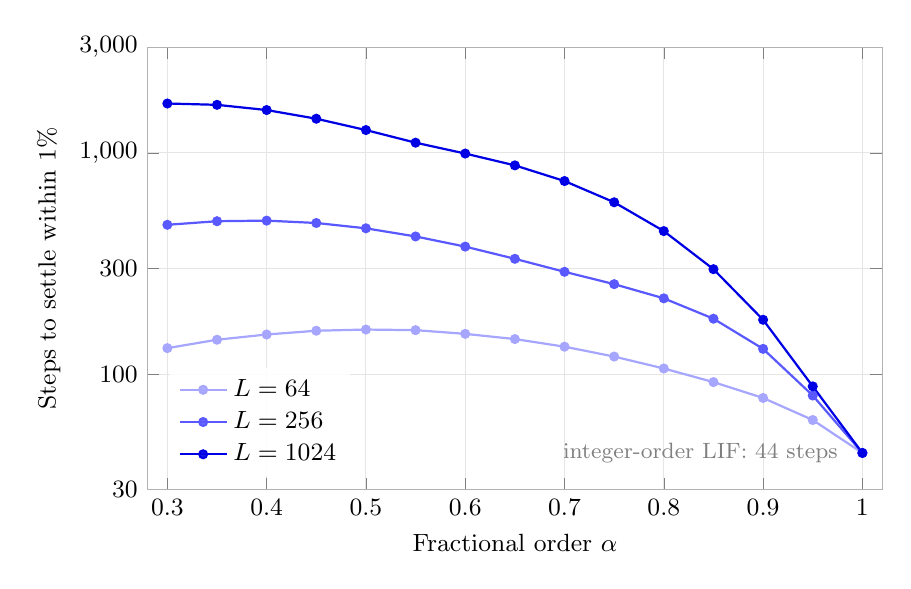
\begin{tikzpicture}
\begin{semilogyaxis}[
  width=0.9\textwidth, height=7.2cm,
  xmin=0.28, xmax=1.02, ymin=30, ymax=3000,
  xlabel={Fractional order $\alpha$},
  ylabel={Steps to settle within 1\%},
  xtick={0.3,0.4,0.5,0.6,0.7,0.8,0.9,1.0},
  ytick={30,100,300,1000,3000},
  yticklabels={30,100,300,1{,}000,3{,}000},
  grid=major, grid style={gray!20},
  axis line style={gray!60},
  tick label style={font=\small},
  label style={font=\small},
  legend style={font=\small, draw=none, fill=none, at={(0.03,0.03)}, anchor=south west, fill=white, fill opacity=0.9, text opacity=1},
  legend cell align=left,
  every axis plot/.append style={thick, mark=*, mark size=1.4pt},
]
\addplot[color=blue!35] coordinates {(0.3,131) (0.35,143) (0.4,151) (0.45,157) (0.5,159) (0.55,158) (0.6,152) (0.65,144) (0.7,133) (0.75,120) (0.8,106) (0.85,92) (0.9,78) (0.95,62) (1.0,44)};
\addlegendentry{$L = 64$}
\addplot[color=blue!65] coordinates {(0.3,473) (0.35,491) (0.4,494) (0.45,482) (0.5,456) (0.55,419) (0.6,377) (0.65,332) (0.7,290) (0.75,255) (0.8,220) (0.85,178) (0.9,130) (0.95,80) (1.0,44)};
\addlegendentry{$L = 256$}
\addplot[color=blue!90!black] coordinates {(0.3,1672) (0.35,1649) (0.4,1562) (0.45,1427) (0.5,1268) (0.55,1112) (0.6,993) (0.65,878) (0.7,746) (0.75,598) (0.8,443) (0.85,298) (0.9,176) (0.95,88) (1.0,44)};
\addlegendentry{$L = 1024$}
\node[anchor=east, font=\footnotesize, text=gray] at (axis cs:0.985,44) {integer-order LIF: 44 steps};
\end{semilogyaxis}
\end{tikzpicture}
\caption{For $\tau_m = 10$ steps a fault lingers for at most about $2.5L$ steps, and short buffers peak at intermediate $\alpha$. Steps to settle within 1\% of the new state after a permanent step-like fault, by GL buffer length $L$. Simulated scalar GL-FLIF step response (Algorithm~1 of~\cite{mastin2026} without threshold), $\Delta t = 1$, $\tau_m = 10$ steps.}
\label{fig:recovery}
\end{figure}

With a long buffer ($L = 1024$), lower $\alpha$ always means slower recovery (Figure~\ref{fig:recovery}). With a short buffer ($L = 64$), the truncation leak dominates at low $\alpha$, so recovery time peaks near $\alpha \approx 0.5$. In every case it stays below about $2.5L$ steps, against the untruncated 318{,}000 at $\alpha = 0.5$.

The ratio to $L$ is specific to $\tau_m = 10$ steps. Once the buffer is truncated, the slowest decay of a real mode $\lambda < 0$ is set by the pole of $H_\lambda(z)$ (Eq.~\eqref{eq:zdomain}) on the real axis closest to $z = 1$, that is, the real root $z^{*}$ of $C_L(z) = \Delta t^{\alpha} \lambda z^{-1}$, which gives a time constant of $-1/\ln z^{*}$ steps. The 1\% recovery time is then at most about
\begin{equation}
T_{1\%} \lesssim \min\left( T_{\varepsilon},\; \frac{\ln 100}{|\ln z^{*}|} \right),
\label{eq:Tcap}
\end{equation}
with $T_{\varepsilon}$ from Eq.~\eqref{eq:Teps} at $\varepsilon = 1\%$. In simulations over $\tau_m \in \{10, 100\}$ steps, $L \in \{64, 256, 1024\}$ and $\alpha$ from 0.3 to 1, this estimate never fell below the simulated recovery time and overestimated it by at most a factor of 1.7. The cap grows with $\tau_m$. At $\alpha = 1$ it is $\tau_m \ln 100 \approx 4.6\,\tau_m$ whatever $L$ is, and for $\tau_m = 100$ steps and $L = 64$ recovery takes up to $8.4L$ (537 steps at $\alpha = 0.9$). The figure's cap of about $2.5L$ therefore does not transfer to other membrane time constants; for the hardware, evaluate Eq.~\eqref{eq:Tcap} at its own $\tau_m$.

\subsection{Check in a network}

The exponents were checked in a linear GL network of 100 neurons with random Gaussian coupling ($g\tau_m = 0.8$), $\tau_m = 2$ steps, $L = 6000$, and an F-all fault at step 3000. The transient fault removed the neuron for 20 steps. For the permanent fault, the slope of $d\delta/dt$ was fitted, which should scale as $t^{-1-\alpha}$. Fits used 300 to 2500 steps after the fault (Table~\ref{tab:exponents}).

\begin{table}[h]
\centering
\small
\begin{tabular}{@{}cccc@{}}
\toprule
$\alpha$ & Predicted exponent & Permanent fault, fitted & Transient fault, fitted \\
\midrule
0.4 & $-1.4$ & $-0.95$ & $-1.20$ \\
0.6 & $-1.6$ & $-1.54$ & $-1.63$ \\
0.8 & $-1.8$ & $-1.81$ & $-1.90$ \\
\bottomrule
\end{tabular}
\caption{Predicted and fitted power-law exponents after a single-neuron fault.}
\label{tab:exponents}
\end{table}

The $\alpha = 0.4$ mismatch is expected: the asymptotic form needs $|\lambda| t^{\alpha} \gg 1$, that is $t \gg |\lambda|^{-1/\alpha} \approx 316$ steps for the slowest mode, which is where the fit window begins. Low-$\alpha$ experiments will need long observation windows to see the predicted tail.

%=====================================================================
\section{Where the reservoir settles}
\label{sec:settle}

At a fixed operating point, the fault's shift of the mean operating point does not depend on $\alpha$, but its effect on how the reservoir responds to inputs does. Removing a random neuron also slightly shrinks the reservoir's spectrum, pushing it toward the ordered regime.

\subsection{The mean shift is independent of \texorpdfstring{$\alpha$}{alpha}}

The fractional derivative of a constant is zero (in the GL form because $\sum_k c_k = 0$), so every $\alpha$ has the same fixed point. For the constant part of the forcing in Eq.~\eqref{eq:pert}, the new steady state of the survivors is
\begin{equation}
\delta^{*} = A'^{-1} q_j\, r_j \quad (L \to \infty), \qquad \delta^{*}_L = \left(A' - \tfrac{\varepsilon_L}{\Delta t^{\alpha}} \mathrm{Id}\right)^{-1} q_j\, r_j \quad (\text{truncated}).
\label{eq:dstar}
\end{equation}
In words: given the operating point, $\alpha$ changes the path to the new operating point, not the point itself, unless the buffer is truncated. On the FPGA, $\alpha$ and $L$ reach the endpoint through the effective leak $\varepsilon_L$.

The operating point itself is a different matter. The rates $r$ and gains $\gamma$, and therefore $A'$, come from the noise-averaged $f$--$I$ curve, which depends on $\alpha$ (lower $\alpha$ raises the effective rheobase~\cite{mastin2026}). In a spiking reservoir the measured $\delta^{*}$ therefore changes with $\alpha$ through $r_j$ and $A'$, even though Eq.~\eqref{eq:dstar} has no explicit $\alpha$. The $\alpha$-independence is a statement about Eq.~\eqref{eq:dstar} at fixed $(r, \gamma)$, and that is how it should be tested.

The fluctuations are different. The surviving reservoir's frequency response is $H'(\omega) = \left((i\omega)^{\alpha} \mathrm{Id} - A'\right)^{-1}$, which depends on $\alpha$ at every frequency except zero. So the information-carrying part of the fault's effect is $\alpha$-dependent even though the mean shift is not.

\subsection{Spectral effect of removing a neuron}

For a specific neuron, first-order perturbation theory gives the shift of each eigenvalue $\lambda_i$, using its left and right eigenvectors $v_i$ and $u_i$ and the change $\Delta A$ from deleting row and column $j$:
\begin{equation}
\delta\lambda_i \approx \frac{v_i^{*}\, \Delta A\, u_i}{v_i^{*} u_i}, \qquad |\delta\lambda_i| \le \kappa(U)\, \|\Delta A\| \le \kappa(U)\left( \|\Wt_{:,j}\| + \|\Wt_{j,:}\| \right).
\label{eq:bauerfike}
\end{equation}
The bound is Bauer--Fike~\cite{bauerfike1960}, with $\kappa(U)$ the condition number of the eigenvector matrix. Neurons with large incoming and outgoing weight norms, and large components in the slowest modes, are the ones whose removal moves the spectrum most.

For a random reservoir the average effect is simple. If $\Wt$ has i.i.d.\ entries of variance $g^2/N$, its eigenvalues fill a disk of radius $g$ (the circular law~\cite{taovu2010}). Deleting $k$ neurons leaves an $(N-k)$-square matrix with the same entry variance, so
\begin{equation}
g_{\mathrm{eff}} = g\sqrt{1-p}, \qquad p = k/N.
\label{eq:geff}
\end{equation}
Here $N$, $k$ and $p$ count active neurons only. A neuron far below threshold has $\gamma_j = 0$, so its column of $\Wt$ is zero and it does not contribute to the spectrum; removing it leaves $g$ unchanged. If $\gamma$ varies across neurons, the columns of $\Wt$ have different variances and the radius is set by their average~\cite{aljadeff2015}: $g^2 = N_{\mathrm{act}}\, \sigma_W^2 \langle \gamma_j^2 \rangle$, with $\sigma_W^2$ the entry variance of $W$ and the average taken over the $N_{\mathrm{act}}$ active neurons.

Random dropout therefore makes the reservoir more stable and more strongly damped. The linearized reservoir loses stability when its eigenvalue disk reaches the leak, at $g\tau_m = 1$. In random rate networks this is also where chaos begins~\cite{sompolinsky1988}, and the transition persists with excitatory--inhibitory structure~\cite{kadmon2015}. Input drive moves the onset of chaos to larger gain~\cite{rajan2010}, so in a driven reservoir the edge of chaos lies somewhat above $g\tau_m = 1$. Either way, losing neurons lowers $g\tau_m$ and moves the reservoir into the ordered regime. With noise, memory capacity should fall too, since driven random networks compute best near this boundary~\cite{bertschinger2004}; in the noise-free linear model it does not (Section~\ref{sec:info}). A single removal changes $g$ by only about $g/(2N)$, so this matters for cumulative faults, not single ones.

\subsection{Stability}

The continuous linear FOR is stable when every eigenvalue satisfies $|\arg\lambda| > \alpha\pi/2$ (Matignon's criterion~\cite{matignon1996}). Smaller $\alpha$ widens the stable sector into the right half-plane, so a fault that pushes a complex eigenvalue pair rightward can leave a low-$\alpha$ reservoir stable when an integer-order one would not be.

This protection does not extend to real eigenvalues. A real eigenvalue crossing zero destabilizes every $\alpha$, and for circular-law reservoirs the first crossing is on the real axis at $g\tau_m = 1$. So $\alpha$ does not move the critical gain of a random reservoir; it only adds margin against faults that act on oscillatory modes.

Near criticality $\alpha$ does amplify the fault's effect on time scales. A mode near zero relaxes on the time scale $|\lambda|^{-1/\alpha}$, so
\begin{equation}
\frac{d \ln T_{\lambda}}{d \ln |\lambda|} = -\frac{1}{\alpha}.
\end{equation}
A fault that shifts a slow eigenvalue by a given fraction changes that mode's time scale by twice that fraction at $\alpha = 0.5$, and by the same fraction at $\alpha = 1$.

In a chaotic reservoir ($g\tau_m>1$) linear response breaks down entirely, and single-neuron clamping can be catastrophic~\cite{vincentlamarre2016}. This analysis assumes the input-driven, echo-state regime.

%=====================================================================
\section{Information-theoretic consequences}
\label{sec:info}

In the linear, noise-free limit with a retrained readout, removing a neuron costs exactly one unit of memory capacity, whatever the value of $\alpha$. Every $\alpha$-dependence in the fault tolerance of the three measures of~\cite{mastin2026} therefore comes from noise, nonlinearity or truncation. In all three, the key quantity is the neuron's \emph{unique variance}, $\Var(x_j \mid x_{-j})$: the part of its state that no other neuron predicts.

The results below assume the linear FOR with Gaussian input or a large-$N$ Gaussian approximation, so that the measures of~\cite{mastin2026} (their Eqs.~8, 11 and~12) have closed forms. $C = \Cov(x)$ is the state covariance and $\sigma_u^2$ the input variance.

\subsection{Memory capacity, readout retrained}

Linear memory capacity at lag $k$ is $MC_k = r_k^{\top} C^{-1} r_k / \sigma_u^2$, with $r_k = \Cov(x_t, u_{t-k})$. Dropping neuron $j$ as a regressor costs exactly
\begin{equation}
\Delta MC_k^{\mathrm{readout}} = \frac{\beta_{kj}^{2}}{(C^{-1})_{jj}\,\sigma_u^{2}} = \frac{\beta_{kj}^{2}\; \Var(x_j \mid x_{-j})}{\sigma_u^{2}}, \qquad \beta_k = C^{-1} r_k.
\label{eq:dmc}
\end{equation}
That is the neuron's readout weight for lag $k$ squared, times its unique variance. Summing over lags, with $S = \sum_k r_k r_k^{\top} / \sigma_u^2$ the input-explained part of $C$,
\begin{equation}
\sum_k \Delta MC_k^{\mathrm{readout}} = \frac{e_j^{\top} C^{-1} S\, C^{-1} e_j}{(C^{-1})_{jj}} \;\le\; 1, \qquad \text{with equality when } S = C.
\label{eq:dmcsum}
\end{equation}
$S = C$ holds for a noise-free linear reservoir driven by i.i.d.\ input. There the faulty $(N-1)$-neuron network also generically keeps $MC = N-1$ (memory capacity is bounded by the number of units~\cite{jaeger2002}), so the total loss including the propagated channel is exactly 1, independent of $\alpha$. With state noise (for example fixed-point quantization, or the spike-count fluctuations dropped by the linearization), $S < C$ and the loss falls below 1 by an $\alpha$-dependent amount.

Table~\ref{tab:mc} shows a numerical check on six random linear GL networks ($N = 10$, $g\tau_m = 0.7$, $\tau_m = 4$ steps, $L = 400$, state noise $\sigma = 10^{-3}$, 300 lags, one random neuron removed).

\begin{table}[h]
\centering
\small
\begin{tabular}{@{}ccccc@{}}
\toprule
$\alpha$ & MC, intact & Loss, readout only & Loss, whole faulty network & Relative loss \\
\midrule
1.0 & 6.32 & $0.18 \pm 0.10$ & $0.41 \pm 0.38$ & 6.4\% \\
0.7 & 5.30 & $0.08 \pm 0.04$ & $0.24 \pm 0.16$ & 4.4\% \\
0.5 & 4.78 & $0.05 \pm 0.02$ & $0.23 \pm 0.16$ & 4.8\% \\
\bottomrule
\end{tabular}
\caption{Memory-capacity loss from removing one neuron, with a retrained readout (mean $\pm$ s.d.\ over six networks).}
\label{tab:mc}
\end{table}

Without noise, one network lost 1.01, 0.95 and 0.79 units at $\alpha = 1$, 0.7 and 0.5. The low-$\alpha$ shortfall from 1 is memory held at lags beyond the 300-lag window, as predicted.

Two things stand out. First, the propagated channel (whole-network loss minus readout-only loss) costs 1.3 to 3.6 times as much as the readout channel, and the ratio grows as $\alpha$ falls, consistent with long memory spreading the fault through the network. Second, lower $\alpha$ loses less capacity in absolute terms but also starts with less, and the relative difference is within the spread. Six small networks are only indicative.

\subsection{Output error, readout fixed}

In the online setting the readout is not retrained, so what matters is the output error. After the transient, its power is
\begin{equation}
\E[e^{2}] = \int \left| w'^{\top} H'(\omega) B' - w^{\top} H(\omega) B \right|^{2} S_u(\omega)\, \frac{d\omega}{2\pi} \; + \; \left( w'^{\top} \delta^{*} - w_j \xb_j \right)^{2}.
\label{eq:errpower}
\end{equation}
The second term is the bias from the mean shift and, at a fixed operating point, is $\alpha$-independent for an untruncated buffer. During the transient it is replaced by $(w'^{\top}\delta(t) - w_j\xb_j)^2$, which carries the power-law tail of the recovery dynamics.

\subsection{Information transfer}

By the chain rule of mutual information, the information transfer $T = I(\upast; X_t)$ of~\cite{mastin2026} splits cleanly into a direct and a propagated loss:
\begin{equation}
\Delta T = \underbrace{I(\upast; X_j \mid X_{-j})}_{\text{direct: unique information}} + \underbrace{I(\upast; X_{-j}) - I(\upast; X'_{-j})}_{\text{propagated}}.
\label{eq:dT}
\end{equation}
In the Gaussian model the direct term has a closed form, using $C_{\xi} = \Cov(x \mid U)$, the noise covariance:
\begin{equation}
I(\upast; X_j \mid X_{-j}) = \tfrac{1}{2} \ln \frac{\Var(x_j \mid x_{-j})}{\Var(x_j \mid x_{-j}, \upast)} = \tfrac{1}{2} \ln \frac{(C_{\xi}^{-1})_{jj}}{(C^{-1})_{jj}}.
\label{eq:cmi}
\end{equation}
The same unique variance governs both this term and the memory-capacity loss. The propagated term has no fixed sign: removing a neuron also removes the noise it injected into the others.

\subsection{Active information storage}

For a stationary Gaussian reservoir, the active information storage $\mathrm{AIS} = I(X_t; X_{t+1})$~\cite{lizier2012} is
\begin{equation}
\mathrm{AIS} = \tfrac{1}{2} \ln \frac{\det C_0}{\det\!\left( C_0 - C_1 C_0^{-1} C_1^{\top} \right)}, \qquad C_1 = \Cov(X_{t+1}, X_t).
\label{eq:ais}
\end{equation}
Two cautions apply. During the recovery transient the reservoir is not stationary, and a deterministic drift is itself predictable, so windowed AIS estimates will be inflated; subtract the mean trajectory (estimated across input realizations) first. And because dropout lowers the effective coupling, $g\sqrt{1-p}$, it weakens the recurrent dominance that~\cite{mastin2026} associate with high AIS. Cumulative dropout should therefore lower AIS and shift the reservoir toward the input-driven end of their trade-off. That is a hypothesis to test, not a result.

\subsection{Redundancy and the correlation peak}

Mastin et al.~\cite{mastin2026} report that neuron-to-neuron correlations peak in the transition region of $\alpha$. Higher correlation means smaller unique variance, so the theory predicts that the \emph{readout channel} of a single-neuron fault is cheapest near that transition. Strong correlation also implies strong coupling, which enlarges the \emph{propagated channel}. Which effect wins is an open question, and measuring both channels separately across $\alpha$ would answer it directly.

%=====================================================================
\section{Spiking-specific effects}

The linear theory holds while every neuron stays in its operating regime. Thresholds add three effects it cannot capture: neurons switching on or off, cascades of such switches, and a deafened neuron that keeps firing.

\subsection{Threshold crossings}
\label{sec:threshold}

Removing neuron $j$ changes the mean input of each postsynaptic neuron $i$ by $-W_{ij} r_j$. Whether $i$'s response stays linear depends on where $\bar I_i$ sits on its noise-averaged $f$--$I$ curve, so the criterion is stated in input units. For an active neuron, the mean free potential $\bar V_i$ lies above $V_{\mathrm{th}}$, and the distance from it to threshold carries no information.
\begin{itemize}
  \item \textbf{Near-silent neurons.} The relevant distance is from $\bar I_i$ to the rheobase. (For a subthreshold neuron this equals $(V_{\mathrm{th}} - \bar V_i)/G_{\mathrm{DC}}$.) If $|W_{ij} r_j|$ exceeds it, $i$ can go silent after losing excitation, or start firing after losing inhibition.
  \item \textbf{Active neurons.} Linear response needs $|W_{ij} r_j|$ to be small compared with the input range over which the slope $f_i'$ changes appreciably.
\end{itemize}
When either condition fails, $i$'s gain $\gamma_i$ jumps, which changes $\Wt$ itself, not just the state.

\subsection{Silencing cascades}

Treat each switch as a branching event. Let $m$ be the expected number of neurons that switch as a direct result of one switch; $m$ depends on the degree, the weight distribution and the distribution of input distances to the rheobase. The expected total number of neurons affected by one fault is then
\begin{equation}
\E[\text{cascade size}] = \frac{1}{1 - m} \quad (m < 1), \qquad m \ge 1 \;\Rightarrow\; \text{macroscopic failure}.
\end{equation}
At $m\ge 1$ a single fault can propagate through the whole network. $\alpha$ enters in two ways. Mastin et al.~\cite{mastin2026} show that lower $\alpha$ raises the effective rheobase, so how $\alpha$ is normalized (bias or input gain) sets the distribution of distances to the rheobase and therefore $m$. And because a fractional neuron answers a step change in drive with a power-law approach, a cascade unfolds more slowly at low $\alpha$: each generation of switches takes longer to complete.

\subsection{The deafened neuron keeps firing}

Under F-in, neuron $j$ loses all input, but two things keep it active:
\begin{itemize}
  \item \textbf{Its GL buffer still holds pre-fault potentials.} Reset writes $V_{\mathrm{reset}}$ into the buffer but leaves older samples in place, so $j$'s potential relaxes toward its bias-driven equilibrium along the fractional step response. It goes on spiking for a while, in an echo of its pre-fault activity that fades as a power law, capped by $L$.
  \item \textbf{Its bias may exceed the rheobase.} If $b$ alone can drive $j$ to threshold, it settles into regular, input-independent firing. The fault then acts as a periodic drive on its downstream neurons, which is narrowband interference rather than silence, and the readout sees a periodic component.
\end{itemize}
So ``deafening'' a fractional neuron is neither instantaneous nor necessarily silent. Whether F-in or F-all is the better model of a real hardware failure depends on where in the circuit the failure sits.

\subsection{Which neurons matter}

Combining the linear results with the spiking picture gives a vulnerability ranking that can be computed from the golden run, before any fault is injected:
\begin{itemize}
  \item \textbf{Direct channel, readout fixed:} $|w_j| \cdot \mathrm{std}(x_j)$.
  \item \textbf{Direct channel, readout retrained:} $\beta_j^2 \cdot \Var(x_j \mid x_{-j})$, from Eq.~\eqref{eq:dmc}.
  \item \textbf{Propagated channel, mean shift:} $\|W_{:,j}\| \cdot r_j$, the lost mean drive of Eq.~\eqref{eq:dstar}, weighted by the slow-mode components of $A'$.
  \item \textbf{Propagated channel, fluctuation:} $\|W_{:,j}\| \cdot \mathrm{std}(z_j)$, weighted the same way. Here $z_j$ is neuron $j$'s recorded spike train passed through the membrane filter,
  \[
  z_{j,n} = \Delta t^{\alpha}\left( -\frac{z_{j,n-1}}{\tau_m} + s_{j,n-1} \right) - \sum_{k=1}^{L} c_k\, z_{j,n-k},
  \]
  the fluctuating drive that $j$ delivered per unit of outgoing weight. It is measured directly rather than through the linear model's $\gamma_j \xtil_j$, which understates it. In the simulated neuron of Section~\ref{sec:linearization}, the measured drive was about five times the linear prediction at $\alpha = 0.5$ and about twice at $\alpha = 1$, because it includes both the response faster than $\gamma_j$ and the spike-train fluctuations the linear model drops~\cite{linsupp}.
  \item \textbf{Cascade risk:} the number of postsynaptic neurons whose mean input lies within $|W_{ij} r_j|$ of the rheobase.
\end{itemize}
Neurons far below threshold ($r_j = 0$, $\gamma_j = 0$) are harmless to remove unless the readout depends on them. A silent neuron near threshold is not covered by this: it sends nothing now, but a fault elsewhere can switch it on.

%=====================================================================
\section{Testable predictions and analysis plan}

The theory yields seven predictions that can be checked against golden-run versus faulty-run differences (Table~\ref{tab:predictions}). The HiL rig produces exactly the quantity the theory is written in, $\delta(t) = x'(t) - x(t)$, because it can replay the same input with and without the fault.

\begin{table}[h]
\centering
\small
\begin{tabularx}{\textwidth}{@{}l>{\raggedright\arraybackslash}X>{\raggedright\arraybackslash}X>{\raggedright\arraybackslash}X@{}}
\toprule
\# & Prediction & How to test & What would falsify it \\
\midrule
P1 & After a permanent fault, $|\delta(t) - \delta^*|$ decays as $t^{-\alpha}$ up to about $L$ steps, then exponentially & Log-log slope of $d\delta/dt$ (about $-1-\alpha$) over a window starting after $|\lambda|^{-1/\alpha}$ steps & Slope independent of $\alpha$, or no break near $L$ \\
P2 & A transient fault decays as $t^{-1-\alpha}$ & Same fit on a fault of a few steps' duration & As P1 \\
P3 & The 1\% recovery time is capped by Eq.~\eqref{eq:Tcap} (about $2.5L$ for $\tau_m = 10$ steps), and peaks at intermediate $\alpha$ for short buffers & Sweep $\alpha$ and $L$ at the hardware's $\tau_m$; compare with Eq.~\eqref{eq:Tcap} and Figure~\ref{fig:recovery} & Recovery time well above Eq.~\eqref{eq:Tcap}, or a monotone curve in $\alpha$ at $L = 64$, $\tau_m = 10$ \\
P4 & At a fixed operating point, the mean shift $\delta^*$ is independent of $\alpha$, apart from the effective leak $\varepsilon_L$ & For each $\alpha$, compare the measured $\delta^*$ with that $\alpha$'s own prediction $A'^{-1} q_j r_j$ (Eq.~\ref{eq:dstar}), using its measured $r$ and $\gamma$, with and without the $\varepsilon_L$ correction & Residual mismatch that varies with $\alpha$ after correction \\
P5 & With a retrained readout, a noise-free linear FOR loses exactly 1 unit of MC per neuron, for every $\alpha$ & Linear GL simulation with long lag windows & Loss that differs from 1 beyond finite-sample bias \\
P6 & Per-neuron damage ranks by the vulnerability scores of the spiking section & Spearman correlation between predicted score and measured loss, over all $N$ single-neuron faults & No correlation \\
P7 & Cumulative random dropout lowers the effective gain as $g\sqrt{1-p}$ and, with noise, memory capacity falls with it & Fit the leading eigenvalues of the faulty linearized network as $p$ grows & Spectral radius that does not shrink with $p$ \\
\bottomrule
\end{tabularx}
\caption{Testable predictions.}
\label{tab:predictions}
\end{table}

\subsection{Plan}

\begin{enumerate}
  \item \textbf{Linear GL network in software.} Confirm P1--P5 and P7 exactly. This is cheap, and every deviation in the later stages can be attributed to spiking or hardware rather than to the theory itself.
  \item \textbf{Spiking GL-FLIF network in software.} Repeat the same faults with the model and normalization of~\cite{mastin2026}. Measure where the linear predictions break, estimate the branching ratio $m$, and test P6. Separate the direct and propagated channels by also running F-out.
  \item \textbf{Fixed-point model.} Quantize states and coefficients to the FPGA's formats. Quantization noise enters as state noise, which per Section~\ref{sec:info} is exactly what makes the memory-capacity loss depend on $\alpha$.
  \item \textbf{HiL.} Inject F-all at a logged cycle, record all neuron states from both the golden and faulty runs, and compute $\delta(t)$, recovery times and the information measures. With the hardware $L$ fixed, P3 says which $\alpha$ values give the slowest recovery.
\end{enumerate}

Use the same estimators as~\cite{mastin2026} for MC, AIS and $T$ so that results compare directly with their Figs.~2 and~3. Their paper does not say which estimator was used for AIS and $T$, so that needs checking with the authors or their code.

%=====================================================================
\section{Limitations and open questions}

The closed-form results are exact for the linear FOR and approximate for the spiking one. The main gaps, and what each one affects:
\begin{itemize}
  \item \textbf{Linearization.} All closed forms assume small perturbations around a stationary asynchronous state. They fail for neurons near threshold, for cascades with $m$ close to 1, and in the chaotic regime.
  \item \textbf{The effective $L$ is not just the buffer length.} Mastin et al.~\cite{mastin2026} (Table~1) show that coefficient precision also truncates the history. With UQ0.16 coefficients the usable history is 699 steps at $\alpha = 0.5$ and 99 at $\alpha = 0.9$. Use whichever of buffer length and precision limit is smaller when computing $\varepsilon_L$.
  \item \textbf{Discrete-time stability.} Matignon's criterion is for continuous time. The explicit GL scheme of Algorithm~1 has its own step-size condition, which should be checked for the $\Delta t$ and $\tau_m$ used on the FPGA.
  \item \textbf{Slow asymptotics at low $\alpha$.} The power-law tails appear only after $|\lambda|^{-1/\alpha}$ steps, which can exceed $L$. At low $\alpha$ the truncated, pre-asymptotic regime may be the only one that is ever observed.
  \item \textbf{Gaussian information measures.} The closed forms for $T$ and AIS assume Gaussian statistics. Spike-train measures need an estimator (binning, Kraskov-type, or a Gaussian approximation on filtered rates), and the estimator used in~\cite{mastin2026} is not stated.
  \item \textbf{Small numerical checks.} The memory-capacity table rests on six networks of ten neurons. It shows the direction of the effects, not their size.
  \item \textbf{Fault scope.} Only whole-neuron removal is treated. Faults in the GL coefficient memory change $\alpha$ for every neuron sharing it and need their own analysis; the same perturbation framework applies, with $\Delta A$ replaced by a change in the kernel $C_L(z)$.
\end{itemize}
The most useful open question for the thesis is the one from the redundancy discussion: across $\alpha$, does the readout channel shrinking near the correlation peak outweigh the propagated channel growing there?

%=====================================================================
\section{Theory versus implementation (SPIRES)}
\label{sec:spires}

The simulations use SPIRES (\href{https://github.com/txmastin/spires}{txmastin/spires}, \texttt{src/neurons/flif\_gl.c} and \texttt{src/reservoir.c}). The formulas above stay as written; these notes record where the implementation differs from the model they assume.
\begin{itemize}
  \item \textbf{Hard threshold, no noise.} Spiking is deterministic (\texttt{V >= V\_th}). The smooth, noise-averaged $f$--$I$ curve can come only from input fluctuations, and with steady input the rate locks to rational values. The $f$--$I$ curve and its slope are therefore measured with the input fluctuations each neuron sees in the golden run (Section~\ref{sec:linearization}), rather than by adding noise to the simulator.
  \item \textbf{Reset matches the model.} Reset overwrites only the current history sample and leaves older samples in place. The actual potential and the free potential therefore obey the same GL recursion with the same input, and their difference is driven only by what the resets remove. Exactly,
\begin{equation*}
V_{j,n} = V^{f}_{j,n} - \sum_{m \le n} \eta_{n-m}\, \kappa_{j,m}, \qquad \eta(z) = \frac{1}{C_L(z) + \Delta t^{\alpha} z^{-1}/\tau_m},
\end{equation*}
where $\kappa_{j,m}$ is the value the update would have produced at step $m$ minus $V_{\mathrm{reset}}$ on steps where the neuron is reset or held, and zero otherwise. The reset kernel $\eta$ is the membrane filter's impulse response, $\eta(z) = H_{\lambda}(z)/\Delta t^{\alpha}$ at $\lambda = -1/\tau_m$ in Eq.~\eqref{eq:zdomain}, so it has the same power-law tail as $G$.
  \item \textbf{Absolute refractory period.} For $t_{\mathrm{ref}}$ after a spike, $V$ is held at $V_{\mathrm{reset}}$ and written to the history each step. The reset becomes a clamp of $n_{\mathrm{ref}}$ steps rather than a single pulse, the rate is capped at $1/(n_{\mathrm{ref}}+1)$ per step, and $\gamma_j$ falls at strong drive. The equation in Eq.~\eqref{eq:glflif} omits $t_{\mathrm{ref}}$. Because the refractory clock accumulates $dt$ by repeated addition, $n_{\mathrm{ref}}$ can come out one step short when $t_{\mathrm{ref}}/dt$ is not exactly representable (for example $dt = 0.1$ and $t_{\mathrm{ref}} = 0.3$ give 2 steps, not 3); with $dt = 1$ and integer $t_{\mathrm{ref}}$ it is exact.
  \item \textbf{Readout state is the post-reset $V$.} \texttt{compute\_output} reads the membrane potential after reset, not the free potential. Treat each reset, with its refractory clamp, as a single pulse of mean size $\bar\kappa_j$, and the spikes by Eq.~\eqref{eq:spikelin}. Then the readout state's fluctuation is $\xtil_j$ passed through the filter $1 - \bar\kappa_j \gamma_j\, \eta(z)$, and its mean is $\bar V_j - \bar\kappa_j\, r_j\, G_{\mathrm{DC}}/\Delta t^{\alpha}$, since $\eta(1) = G_{\mathrm{DC}}/\Delta t^{\alpha}$. The direct-channel and memory-capacity formulas use the free potential; expect deviations from this filter in measured direct losses and MC.
  \item \textbf{Two time scales.} Each input sample is held for $1/dt$ micro-steps, and the readout samples $V$ once per macro-step. Recovery dynamics, $\tau_m$, $t_{\mathrm{ref}}$ and the GL buffer run in micro-steps; MC lags and readout errors are in macro-steps. The numbers in this document assume $dt = 1$, where the two coincide.
  \item \textbf{Buffer length.} The buffer has $T_{\mathrm{mem}}/dt$ slots and the history sum runs to $k = T_{\mathrm{mem}}/dt - 1$, so $L = T_{\mathrm{mem}}/dt - 1$. The truncation leak pulls toward 0, not $V_{\mathrm{rest}}$, which the formula for $\bar V_j$ already includes. History before step 0 is effectively zero, so discard a washout period.
  \item \textbf{One-step spike delay} (confirmed). Neuron $i$ receives $W s_{n-1}$, matching $I_{i,n}$ in Eq.~\eqref{eq:glflif} and the $z^{-1}$ in Eq.~\eqref{eq:zdomain}. Each spike adds $W_{ij}\,dt^{\alpha}$ to $V$.
  \item \textbf{Shared GL coefficients.} All neurons share one coefficient array, so $\alpha$ is uniform and a coefficient-memory fault affects every neuron at once.
  \item \textbf{Assumed settings.} The analysis assumes \texttt{SYNAPSE\_SIMPLE} (other synapse types add a filter $K_{\mathrm{syn}}(z)$ to $\Wt$) and \texttt{PLASTICITY\_NONE} (plasticity would let the golden and faulty runs' weights drift apart).
\end{itemize}

%=====================================================================
\begin{thebibliography}{10}

\bibitem{mastin2026}
T.~Mastin, N.~Anderson, S.~McNeal, M.~Tubbin and C.~Teuscher,
``Fractional-order systems for neuromorphic computing: software and hardware opportunities and challenges,''
\emph{npj Unconventional Computing}, vol.~3, art.~24, 2026.
\href{https://doi.org/10.1038/s44335-026-00070-8}{doi:10.1038/s44335-026-00070-8}.

\bibitem{vincentlamarre2016}
P.~Vincent-Lamarre, G.~Lajoie and J.-P.~Thivierge,
``Driving reservoir models with oscillations: a solution to the extreme structural sensitivity of chaotic networks,''
\emph{Journal of Computational Neuroscience}, vol.~41, pp.~305--322, 2016.
\href{https://doi.org/10.1007/s10827-016-0619-3}{doi:10.1007/s10827-016-0619-3}.

\bibitem{sompolinsky1988}
H.~Sompolinsky, A.~Crisanti and H.~J.~Sommers,
``Chaos in random neural networks,''
\emph{Physical Review Letters}, vol.~61, no.~3, p.~259, 1988.

\bibitem{kadmon2015}
J.~Kadmon and H.~Sompolinsky,
``Transition to chaos in random neuronal networks,''
\emph{Physical Review X}, vol.~5, art.~041030, 2015.
\href{https://doi.org/10.1103/PhysRevX.5.041030}{doi:10.1103/PhysRevX.5.041030}.

\bibitem{rajan2010}
K.~Rajan, L.~F.~Abbott and H.~Sompolinsky,
``Stimulus-dependent suppression of chaos in recurrent neural networks,''
\emph{Physical Review E}, vol.~82, art.~011903, 2010.
\href{https://doi.org/10.1103/PhysRevE.82.011903}{doi:10.1103/PhysRevE.82.011903}.

\bibitem{bertschinger2004}
N.~Bertschinger and T.~Natschl\"ager,
``Real-time computation at the edge of chaos in recurrent neural networks,''
\emph{Neural Computation}, vol.~16, no.~7, pp.~1413--1436, 2004.
\href{https://doi.org/10.1162/089976604323057443}{doi:10.1162/089976604323057443}.

\bibitem{matignon1996}
D.~Matignon,
``Stability results for fractional differential equations with applications to control processing,''
in \emph{Computational Engineering in Systems Applications (CESA '96)}, Lille, France, vol.~2, pp.~963--968, 1996.

\bibitem{podlubny1999}
I.~Podlubny,
\emph{Fractional Differential Equations},
Mathematics in Science and Engineering, vol.~198. San Diego: Academic Press, 1999.

\bibitem{garrappa2015}
R.~Garrappa,
``Numerical evaluation of two and three parameter Mittag-Leffler functions,''
\emph{SIAM Journal on Numerical Analysis}, vol.~53, no.~3, pp.~1350--1369, 2015.
\href{https://doi.org/10.1137/140971191}{doi:10.1137/140971191}.

\bibitem{jaeger2002}
H.~Jaeger,
``Short term memory in echo state networks,''
GMD Report 152, German National Research Center for Information Technology, 2002.

\bibitem{bauerfike1960}
F.~L.~Bauer and C.~T.~Fike,
``Norms and exclusion theorems,''
\emph{Numerische Mathematik}, vol.~2, pp.~137--141, 1960.
\href{https://doi.org/10.1007/BF01386217}{doi:10.1007/BF01386217}.

\bibitem{taovu2010}
T.~Tao and V.~Vu (with an appendix by M.~Krishnapur),
``Random matrices: universality of ESDs and the circular law,''
\emph{Annals of Probability}, vol.~38, no.~5, 2010.
\href{https://doi.org/10.1214/10-AOP534}{doi:10.1214/10-AOP534}.

\bibitem{aljadeff2015}
J.~Aljadeff, M.~Stern and T.~Sharpee,
``Transition to chaos in random networks with cell-type-specific connectivity,''
\emph{Physical Review Letters}, vol.~114, art.~088101, 2015.
\href{https://doi.org/10.1103/PhysRevLett.114.088101}{doi:10.1103/PhysRevLett.114.088101}.

\bibitem{lizier2012}
J.~T.~Lizier, M.~Prokopenko and A.~Y.~Zomaya,
``Local measures of information storage in complex distributed computation,''
\emph{Information Sciences}, vol.~208, pp.~39--54, 2012.
\href{https://doi.org/10.1016/j.ins.2012.04.016}{doi:10.1016/j.ins.2012.04.016}.

\bibitem{linsupp}
``Linearizing the GL-FLIF reservoir: a detailed walkthrough,''
supplement to this document (\texttt{linearization\_supplement.pdf}), 2026.
Simulation code in \texttt{linearization\_supplement\_sim/}.

\end{thebibliography}

\end{document}
